\chapter{Creating Custom Metrics}\label{ch:custom_metrics}

\section{Conceptual Overview} 

\section{Sample Workflow}

In l2metrics/core.py we introduce an abstract Metric class which describes the general format for any Metric you may use or write, whether for Agent or Classification Learners. The most relevant piece of the Metric class is the calculate method, which has the following required arguments: the log data, a phase\_info dataframe, and a metrics\_dict dataframe. The metrics\_dict starts blank and is filled by each metric in its turn, whereas the log data and the phase info are extracted in the MetricsReport constructor from the logs via two helper functions: \\[0.1in]

l2metrics/util.py - (read\_log\_data): scrapes the logs and returns a pandas dataframe of the logs and task parameters\\
l2metrics/\_localutil.py - (parse\_blocks): builds a pandas dataframe of the phase information contained in the log data\\[0.1in]

These dataframes are passed along by the MetricsReport to the appropriate metric and thus the Metrics and MetricsReport classes should be utilized in conjuction with each other. Though there are a list of default metrics which the MetricsReport uses for the Core Capabilties being exercised at this time, you may choose to add your own metric to this list by using the add method on MetricsReport. Please see the calc\_metrics.py file for more details on how to get started with writing your own custom metric. An extremely simple whole-syllabus-mean is currently implemented as an example to help get you started.


\subsection*{Syllabus and Log Files - Assumptions and Requirements}

\textit{Please note:} Log files should be generated automatically and should require no action on the performer's part. However, Single Task Expert JSON files and/or custom syllabi creation rules must be followed or the L2Metrics code may not work.\\[0.1in]


1. Log files \textbf{must} include logged reward, and the column in the data file \textbf{must} be named reward. Without this column, the metrics code will fail. This is assumed to be logged per episode. \\[0.1in]

2. Single Task Expert Saturation values for each task \textbf{must} be included in a JSON file found in \$L2DATA/taskinfo/info.json and without this file, the metric "Comparison to STE" cannot be calculated. Further, the task names contained in the JSON file must match the names in the log files exactly. The format for this file will be: \\[0.1in]

    \{\\
    "task\_name\_1" : 0.8746,\\
    "task\_name\_2" : 0.9315,\\
    ...,\\
    "task\_name\_n" : 0.8089\\
    \}\\[0.1in]

3. Syllabi used to generate the log files \textbf{must} include annotations with phase information and shall conform to the below convention. Please see Figure~\ref{fig:syllabus} for an example\\[0.1in]

\textit{Phase annotation format}:\\[0.1in]
    \{"\$phase":  "1.train"\}, \{"\$phase":  "1.test"\}, \{"\$phase":  "2.train"\}, \{"\$phase":  "2.test"\}, etc\\[0.1in]

\textit{Structure - Continual Learning}:\\[0.1in]

Consists \textbf{only} of a single task with parametric variations exercised throughout the syllabus. Testing phase is optional, but recommended. The purpose of this type of syllabus is to assess whether the agent can adjust to changes in the environment and maintain performance on the previous parameters when new ones are introduced


\subsection*{Getting Started}

Get started by first generating some log files. You may do this by the following:

1. Download and install the minigridkit repo, located here: \textit{PUT A LINK HERE}

2. Configure your environment variable \$L2DATA to wherever you want your logs to end up.

3. Run minigrid\_learnkit/minigrid\_train\_ppo.py

4. Your logs should appear in \$L2DATA\textbackslash logs\textbackslash  "YOUR\_LOG\_DIRECTORY"\\[0.1in]


Then, you should be able to:\\[0.1in]


5. Pass "YOUR\_LOG\_DIRECTORY" as the log\_dir parameter in the calc\_metrics.py file, and you should get an output printed to console that looks something like this: 


\begin{figure}[h]
	\centering
	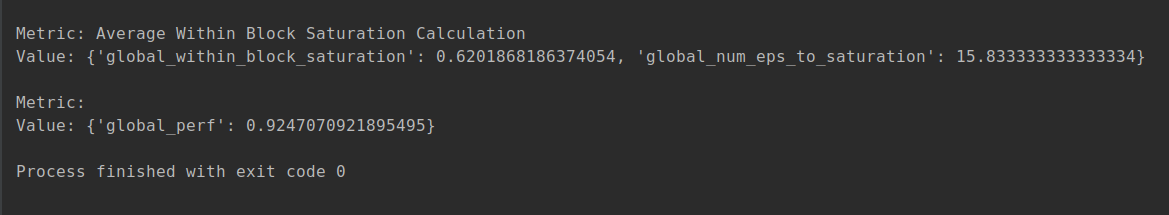
\includegraphics[width=0.85\columnwidth]{sections/figs/calc_metrics_output.png}
	\caption{Sample output for the example calc\_metrics.py .}
	\label{fig:calcmetricsoutput}
\end{figure}

Then, you should be able to:\\[0.1in]


5. Pass "YOUR\_LOG\_DIRECTORY" as the log\_dir parameter in the calc\_metrics.py file, and you should get an output printed to console that looks something like this: 


\begin{figure}[h]
	\centering
	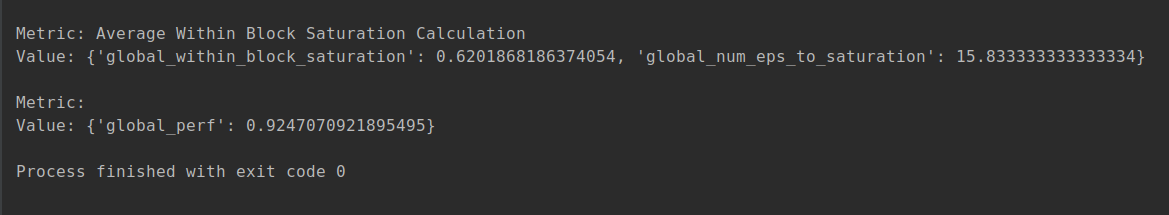
\includegraphics[width=0.85\columnwidth]{sections/figs/calc_metrics_output.png}
	\caption{Sample output for the example calc\_metrics.py .}
	\label{fig:calcmetricsoutput}
\end{figure}
